% ASGARD/Loki draft (verified numbers, humanized)
\section{Results}
\label{sec:results}

\subsection{Main development ablations}
\label{sec:main}

All nine variants completed all three scheduled fits. On outer development, QMMF achieved full-modality group Dice of 0.8052$\pm$0.0028 against 0.8106$\pm$0.0042 for no quality (Table~\ref{tab:main}); no adjusted same-family contrast established a QMMF advantage on any endpoint. The matched moment-fusion control---equal available weights, mean plus dispersion, no learned gate---reached 0.8098$\pm$0.0032 full-modality and a better worst-subset mean, and the paired comparison is decisive: QMMF minus matched-moment worst-subset Dice is $-0.0184$ with adjusted interval $[-0.0335,-0.0035]$. Removing either fusion statistic alone (no-variance 0.8073$\pm$0.0011; no-max 0.8066$\pm$0.0032) leaves full-modality contrasts uncertain, so neither branch is established as necessary.

\begin{table*}[tp]
\centering
\caption{Outer-development segmentation, means$\pm$sample SD over three fixed seeds (27 fits). Group-bootstrap intervals and cohort denominators are in the repository results report; cross-family rows change architecture and auxiliary objective together.}
\label{tab:main}
\begin{tabular}{lccc}
\toprule
Model & Full Dice & Mean-subset Dice & Worst-subset Dice \\
\midrule
QMMF & 0.8052 $\pm$ 0.0028 & 0.6492 $\pm$ 0.0059 & 0.3407 $\pm$ 0.0184 \\
No quality & 0.8106 $\pm$ 0.0042 & 0.6551 $\pm$ 0.0081 & 0.3537 $\pm$ 0.0197 \\
Shuffled quality & 0.8044 $\pm$ 0.0008 & 0.6455 $\pm$ 0.0060 & 0.3246 $\pm$ 0.0323 \\
Matched moment fusion & 0.8098 $\pm$ 0.0032 & 0.6548 $\pm$ 0.0023 & 0.3591 $\pm$ 0.0107 \\
No variance & 0.8073 $\pm$ 0.0011 & 0.6512 $\pm$ 0.0068 & 0.3462 $\pm$ 0.0042 \\
No max & 0.8066 $\pm$ 0.0032 & 0.6528 $\pm$ 0.0077 & 0.3423 $\pm$ 0.0135 \\
No consistency & 0.8043 $\pm$ 0.0038 & 0.6441 $\pm$ 0.0052 & 0.3394 $\pm$ 0.0082 \\
HeMIS-style & 0.7072 $\pm$ 0.0060 & 0.5403 $\pm$ 0.0039 & 0.2338 $\pm$ 0.0249 \\
U-Net 2.5D & 0.7865 $\pm$ 0.0105 & 0.6107 $\pm$ 0.0093 & 0.2912 $\pm$ 0.0196 \\
\bottomrule
\end{tabular}
\end{table*}

Two contrasts separate from the null. QMMF exceeded shuffled quality on worst-subset Dice by $0.0161$ with adjusted interval $[+0.0009,+0.0326]$---mismatched training descriptors are actively harmful---while its full- and mean-subset contrasts with the shuffled control remained uncertain. An advantage over descriptor corruption does not establish benefit over descriptor omission. Second, removing consistency \emph{reduced} mean-subset Dice by $0.0050$ from the control's perspective; equivalently, QMMF minus no-consistency on mean-subset Dice is $+0.0050$ with adjusted interval $[+0.0015,+0.0102]$ (Fig.~\ref{fig:mainablation}), the only same-family contrast that favours a QMMF component, and its full- and worst-subset comparisons were uncertain. No reserved no-consistency run exists, so this effect is measured on development only.

\begin{figure}[htbp]
\centering
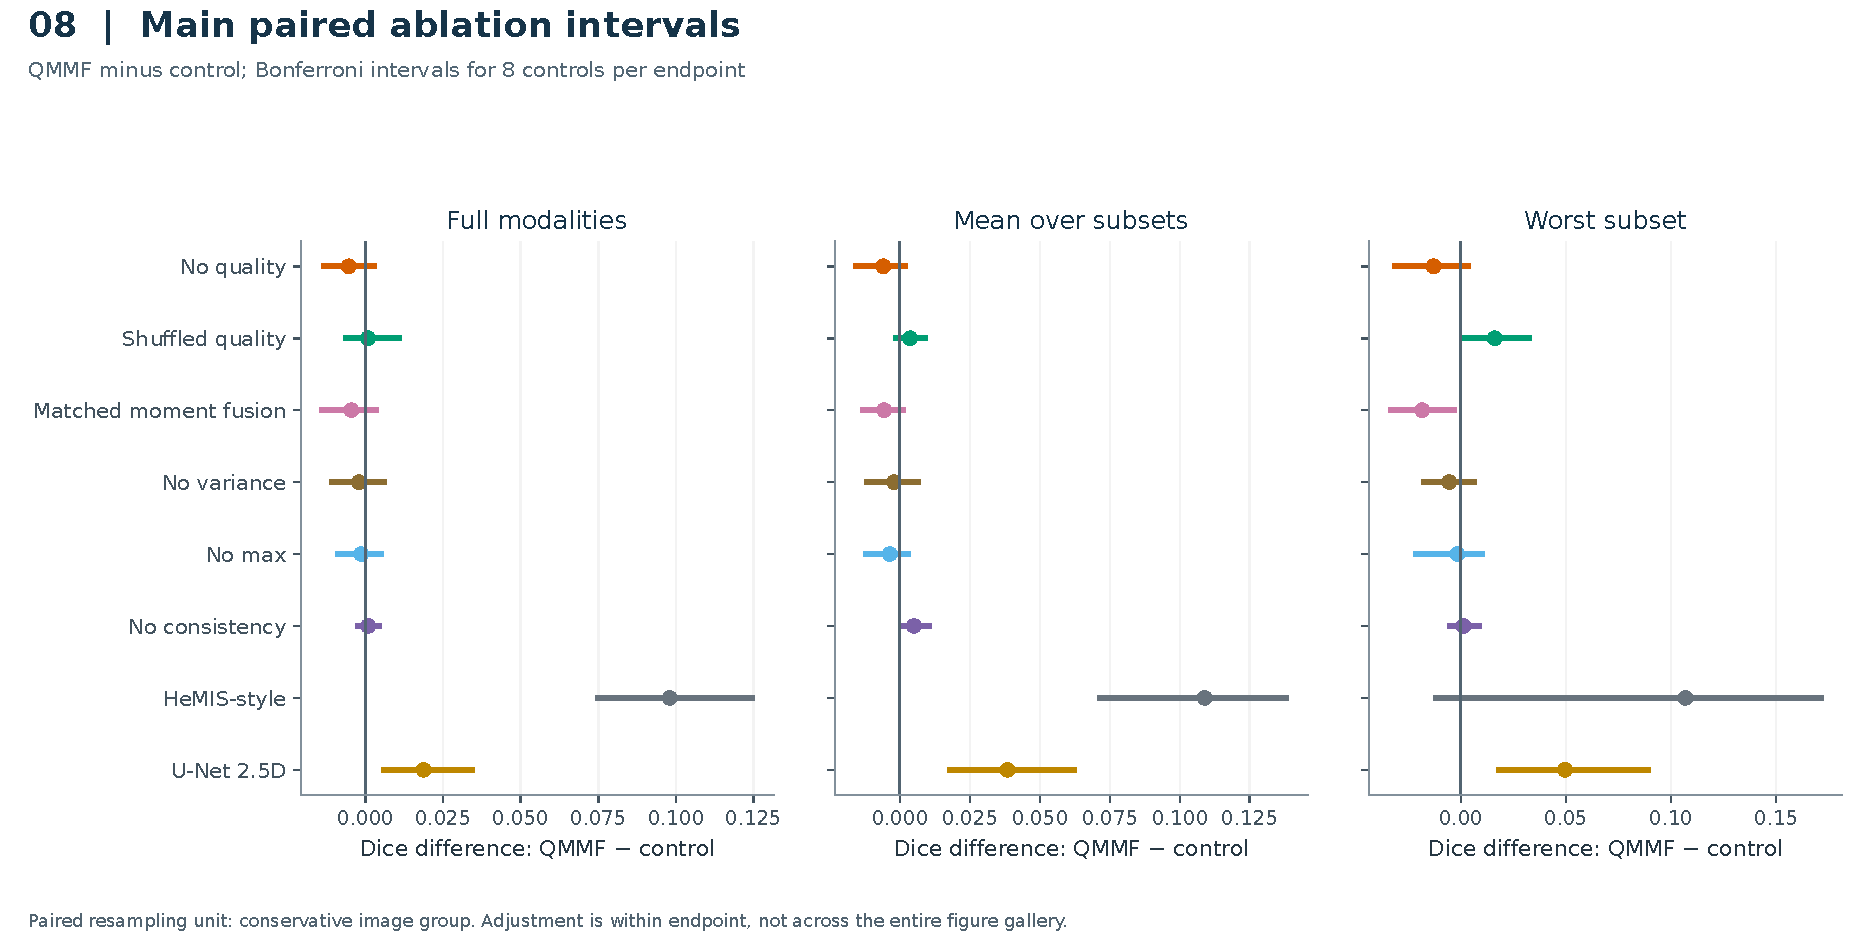
\includegraphics[width=\columnwidth]{figures/fig08_main_paired_ablations.pdf}
\caption{Adjusted paired QMMF--control contrasts on the main development study, all three endpoints, all eight controls. Intervals crossing zero are uncertain; positive favours QMMF.}
\label{fig:mainablation}
\end{figure}

\subsection{Reserved-cohort evaluation}
\label{sec:reserved}

The four prespecified families were evaluated with their three selected checkpoints each, producing 12 completed reserved evaluations on all 66 cases in 51 groups (Table~\ref{tab:reserved}). QMMF reached full-modality group Dice of 0.7689$\pm$0.0055; no quality reached 0.7769$\pm$0.0007. The difference is $-0.0080$ with adjusted interval $[-0.0133,-0.0028]$; mean-subset ($-0.0083$, $[-0.0124,-0.0042]$) and worst-subset ($-0.0214$, $[-0.0322,-0.0119]$) comparisons also favour the control (Table~\ref{tab:contrasts}, Fig.~\ref{fig:reserved}). Under the recorded protocol, the implemented quality descriptors do not earn their place.

\begin{table}[t]
\centering
\caption{Reserved-cohort segmentation (66 cases, 51 groups), means$\pm$sample SD over three seeds (12 checkpoint evaluations).}
\label{tab:reserved}
\scriptsize
\setlength{\tabcolsep}{3.2pt}
\begin{tabular}{lccc}
\toprule
Model & Full Dice & Mean-subset & Worst-subset \\
\midrule
QMMF & 0.7689 $\pm$ 0.0055 & 0.6322 $\pm$ 0.0080 & 0.3672 $\pm$ 0.0120 \\
No quality & 0.7769 $\pm$ 0.0007 & 0.6405 $\pm$ 0.0075 & 0.3886 $\pm$ 0.0137 \\
HeMIS-style & 0.6837 $\pm$ 0.0007 & 0.5462 $\pm$ 0.0080 & 0.2748 $\pm$ 0.0286 \\
U-Net 2.5D & 0.7621 $\pm$ 0.0074 & 0.6034 $\pm$ 0.0078 & 0.3140 $\pm$ 0.0115 \\
\bottomrule
\end{tabular}
\end{table}

\begin{table}[t]
\centering
\caption{Reserved paired contrasts (QMMF$-$control), 10{,}000 group-bootstrap draws retaining all three seeds; Bonferroni adjustment over three controls per endpoint. Negative favours the control.}
\label{tab:contrasts}
\scriptsize
\begin{tabular}{llcc}
\toprule
Control & Endpoint & Diff. & Adjusted interval \\
\midrule
No quality & Full & $-0.0080$ & $[-0.0133,-0.0028]$ \\
No quality & Mean subset & $-0.0083$ & $[-0.0124,-0.0042]$ \\
No quality & Worst subset & $-0.0214$ & $[-0.0322,-0.0119]$ \\
HeMIS-style & Full & $+0.0853$ & $[+0.0712,+0.0993]$ \\
HeMIS-style & Mean subset & $+0.0861$ & $[+0.0734,+0.1003]$ \\
HeMIS-style & Worst subset & $+0.0923$ & $[+0.0617,+0.1258]$ \\
U-Net 2.5D & Full & $+0.0068$ & $[-0.0045,+0.0189]$ \\
U-Net 2.5D & Mean subset & $+0.0289$ & $[+0.0210,+0.0375]$ \\
U-Net 2.5D & Worst subset & $+0.0532$ & $[+0.0355,+0.0738]$ \\
\bottomrule
\end{tabular}
\end{table}

\begin{figure}[htbp]
\centering
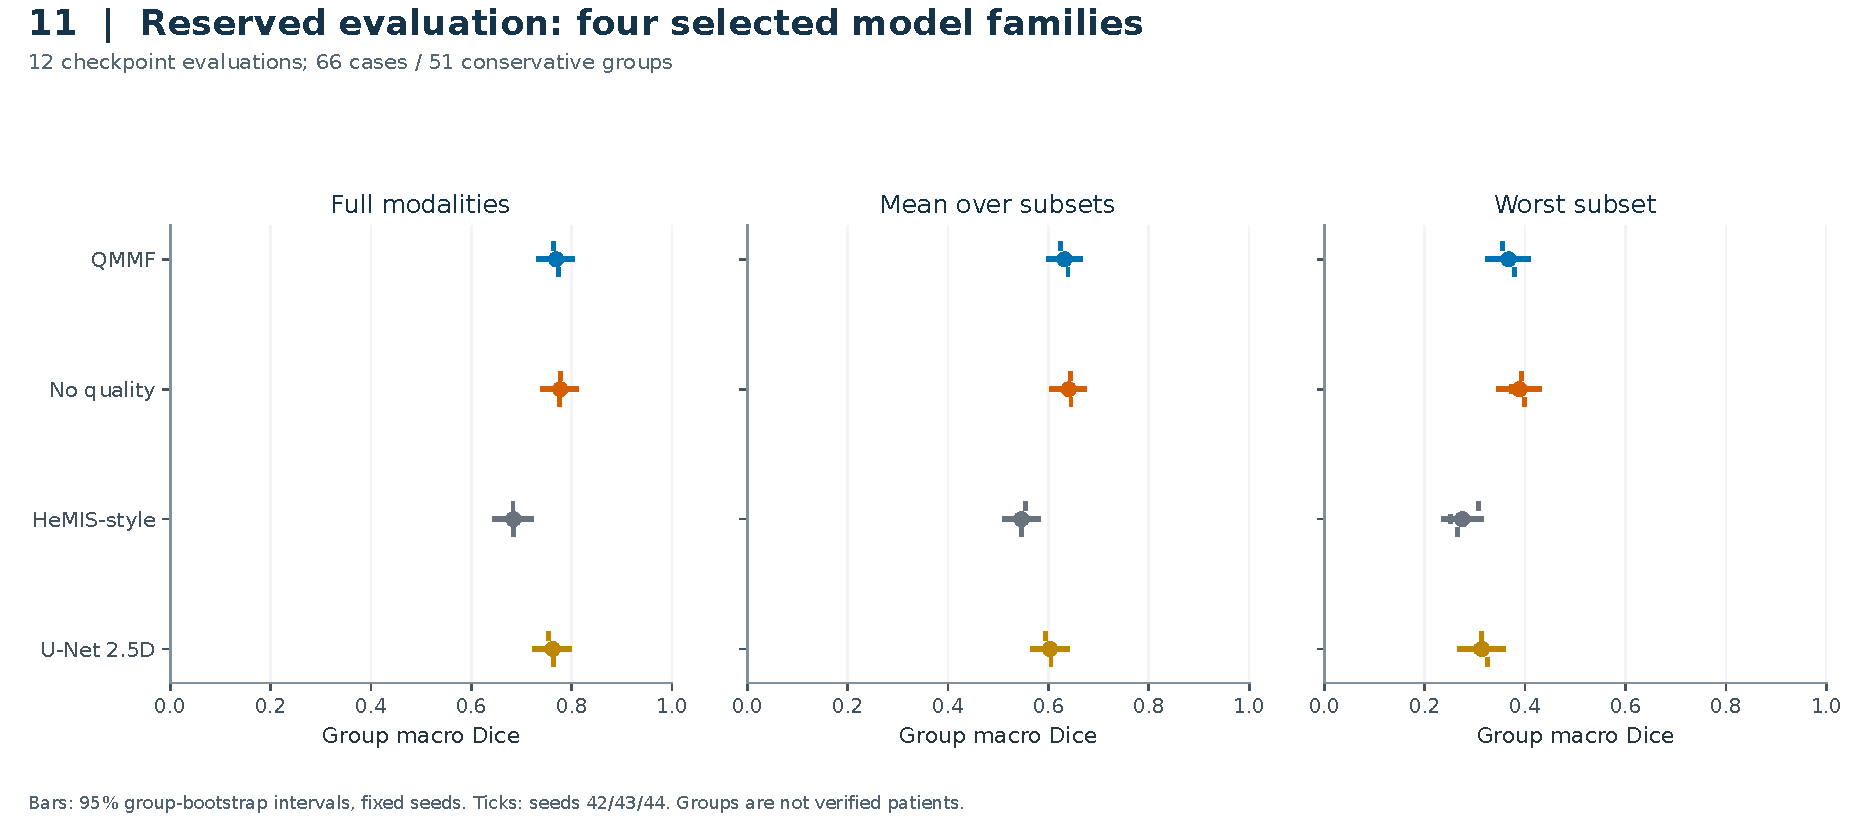
\includegraphics[width=\columnwidth]{figures/fig11_reserved_segmentation_endpoints.pdf}
\caption{Reserved endpoints for all four families, all three seeds: full-modality, mean-subset and worst-subset group Dice.}
\label{fig:reserved}
\end{figure}

\begin{figure}[htbp]
\centering
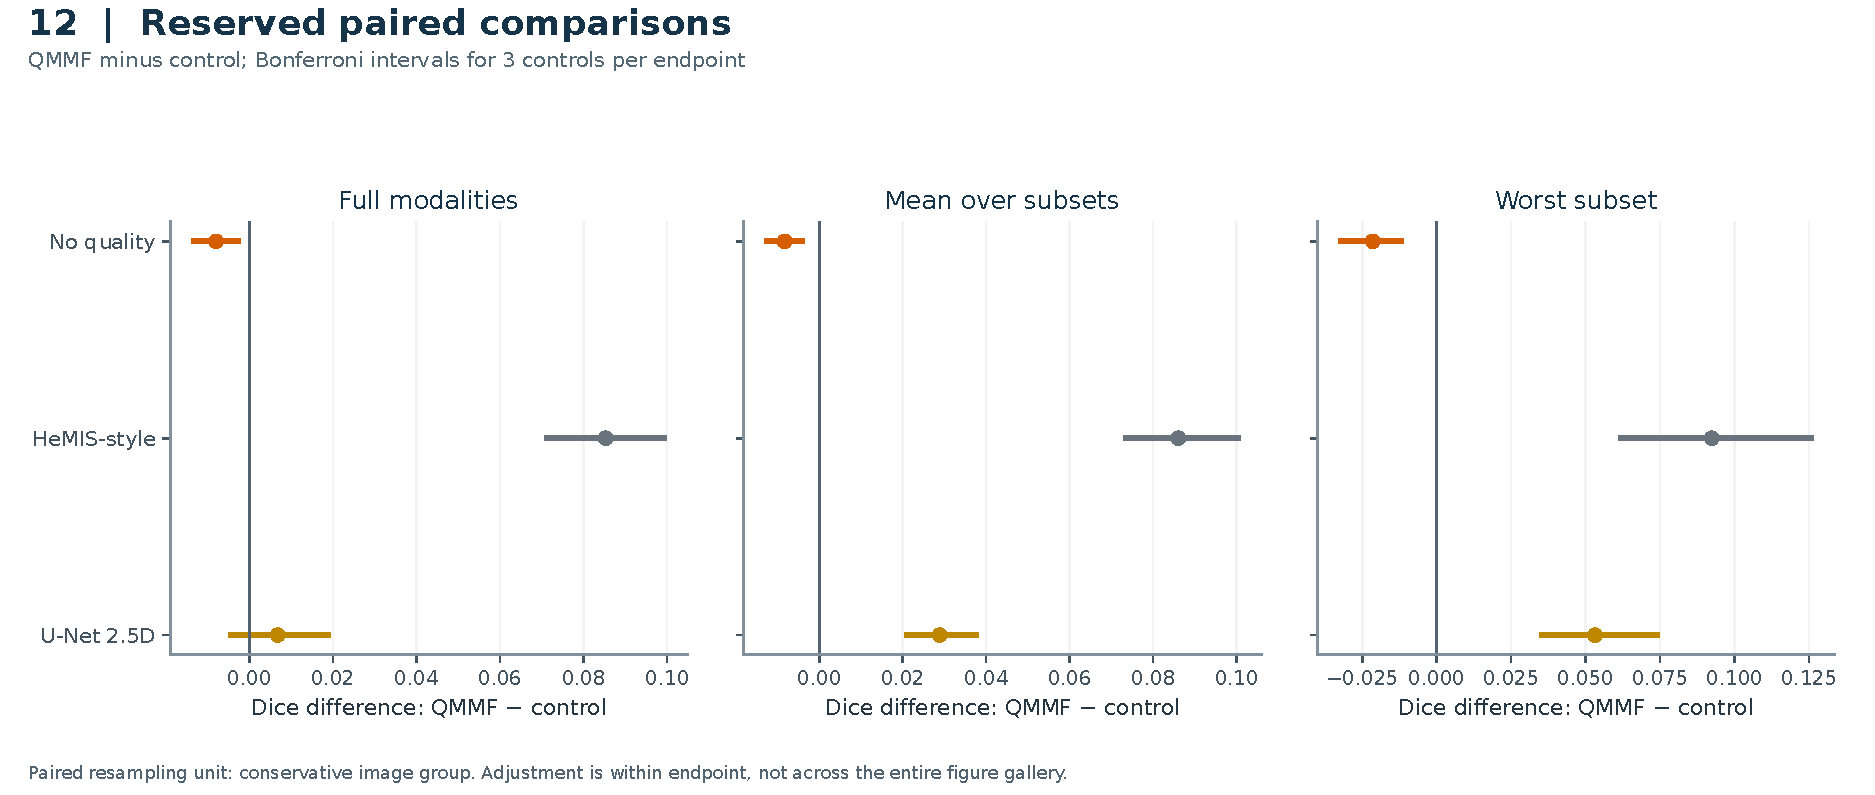
\includegraphics[width=\columnwidth]{figures/fig12_reserved_paired_contrasts.pdf}
\caption{All nine declared reserved paired contrasts with adjusted group-bootstrap intervals.}
\label{fig:reservedcontrasts}
\end{figure}

Across families, QMMF exceeded the HeMIS-style comparator on all three reserved endpoints under the declared adjustment ($+0.0853$ to $+0.0923$), and its full-modality comparison with U-Net 2.5D was uncertain ($+0.0068$, $[-0.0045,+0.0189]$) while subset comparisons favoured QMMF (Fig.~\ref{fig:reservedcontrasts}). These cross-family findings cannot isolate the quality module because architecture and effective auxiliary objective change together; the comparison set was fixed before reserved outcomes and not expanded to whichever variant ranked first.

\subsection{Missing-modality subsets and failure analysis}
\label{sec:subsets}

\begin{figure}[htbp]
\centering
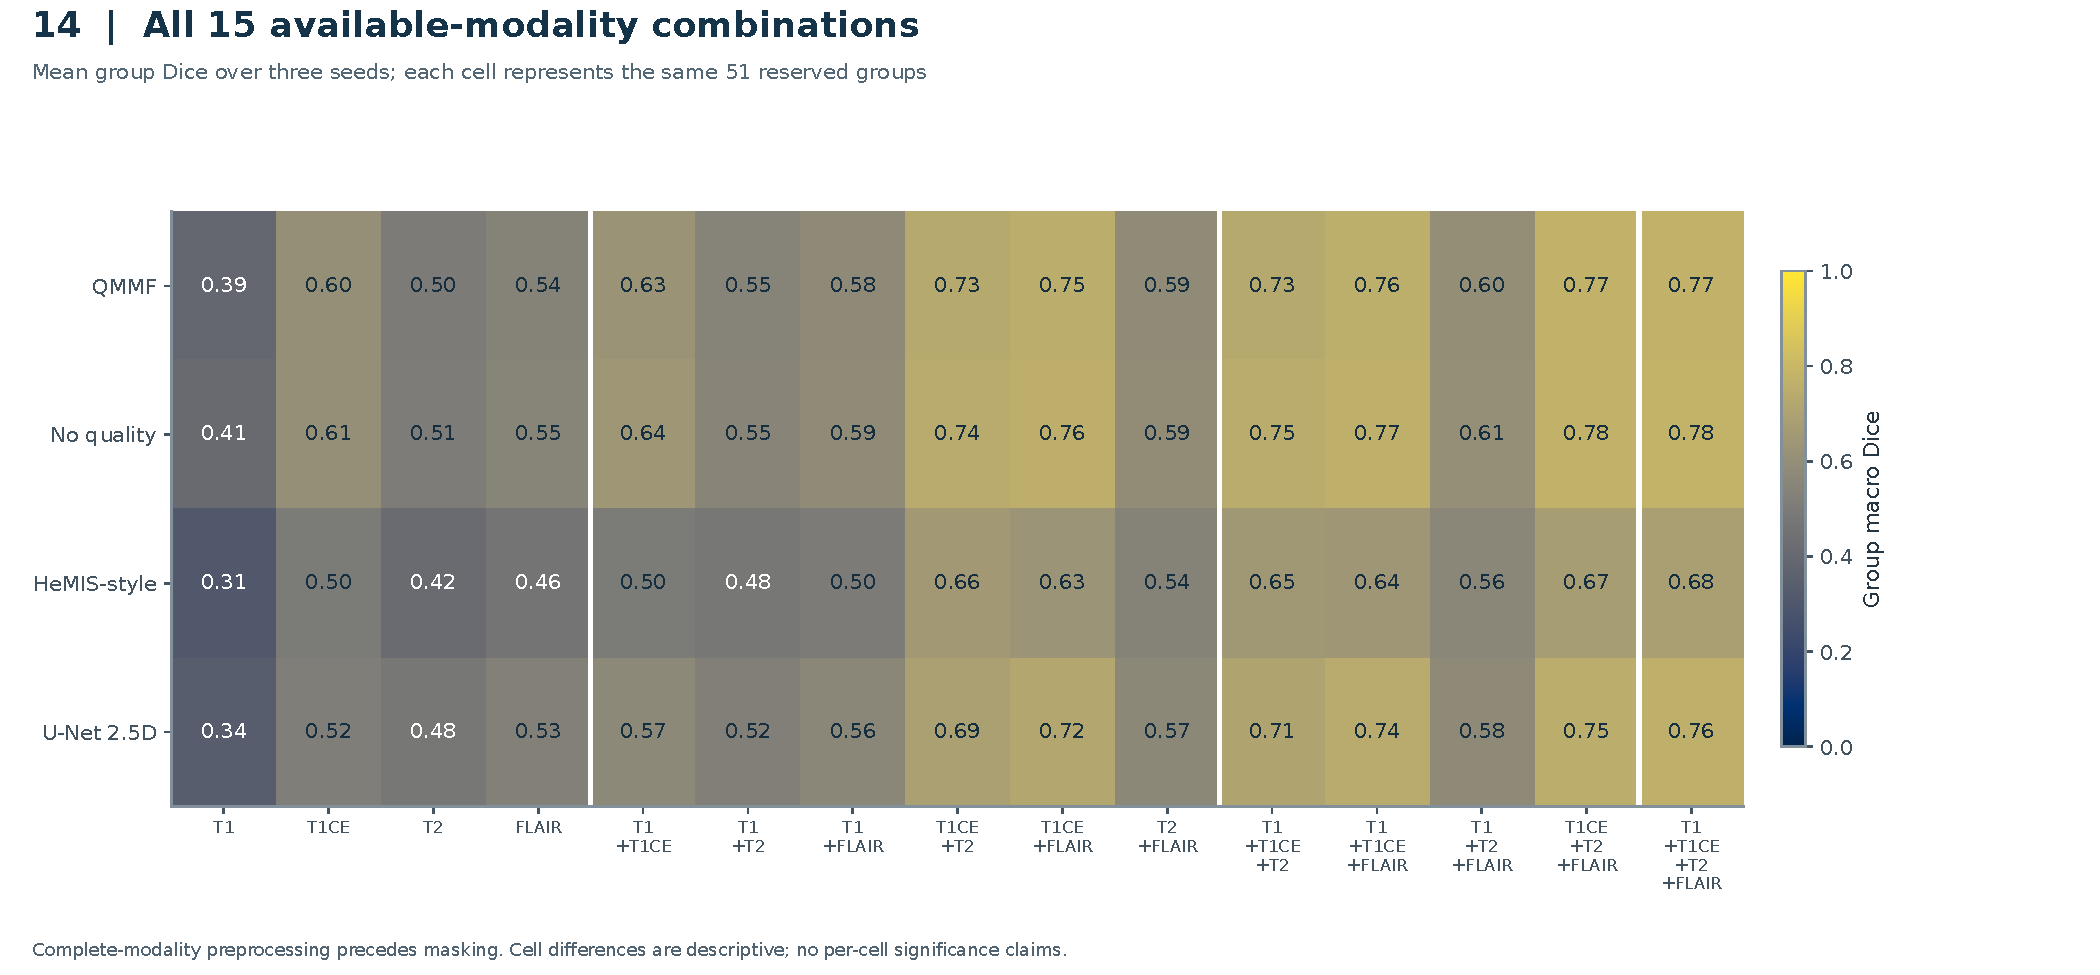
\includegraphics[width=\columnwidth]{figures/fig14_reserved_modality_subsets.pdf}
\caption{Reserved group-macro Dice for all 15 nonempty modality combinations, four models, three seeds (one representative per group). The no-quality control attains the higher descriptive mean in every column.}
\label{fig:subsets}
\end{figure}

Across all 15 modality combinations, the no-quality control held the higher descriptive three-seed mean in every cell; these cell-wise comparisons are not additional adjusted tests. QMMF's T1-alone score was approximately 0.3921, above its average case-specific worst-subset score of 0.3672---a worst-subset mean can sit below every column mean because different cases fail on different combinations (Fig.~\ref{fig:subsets}).

\begin{figure}[htbp]
\centering
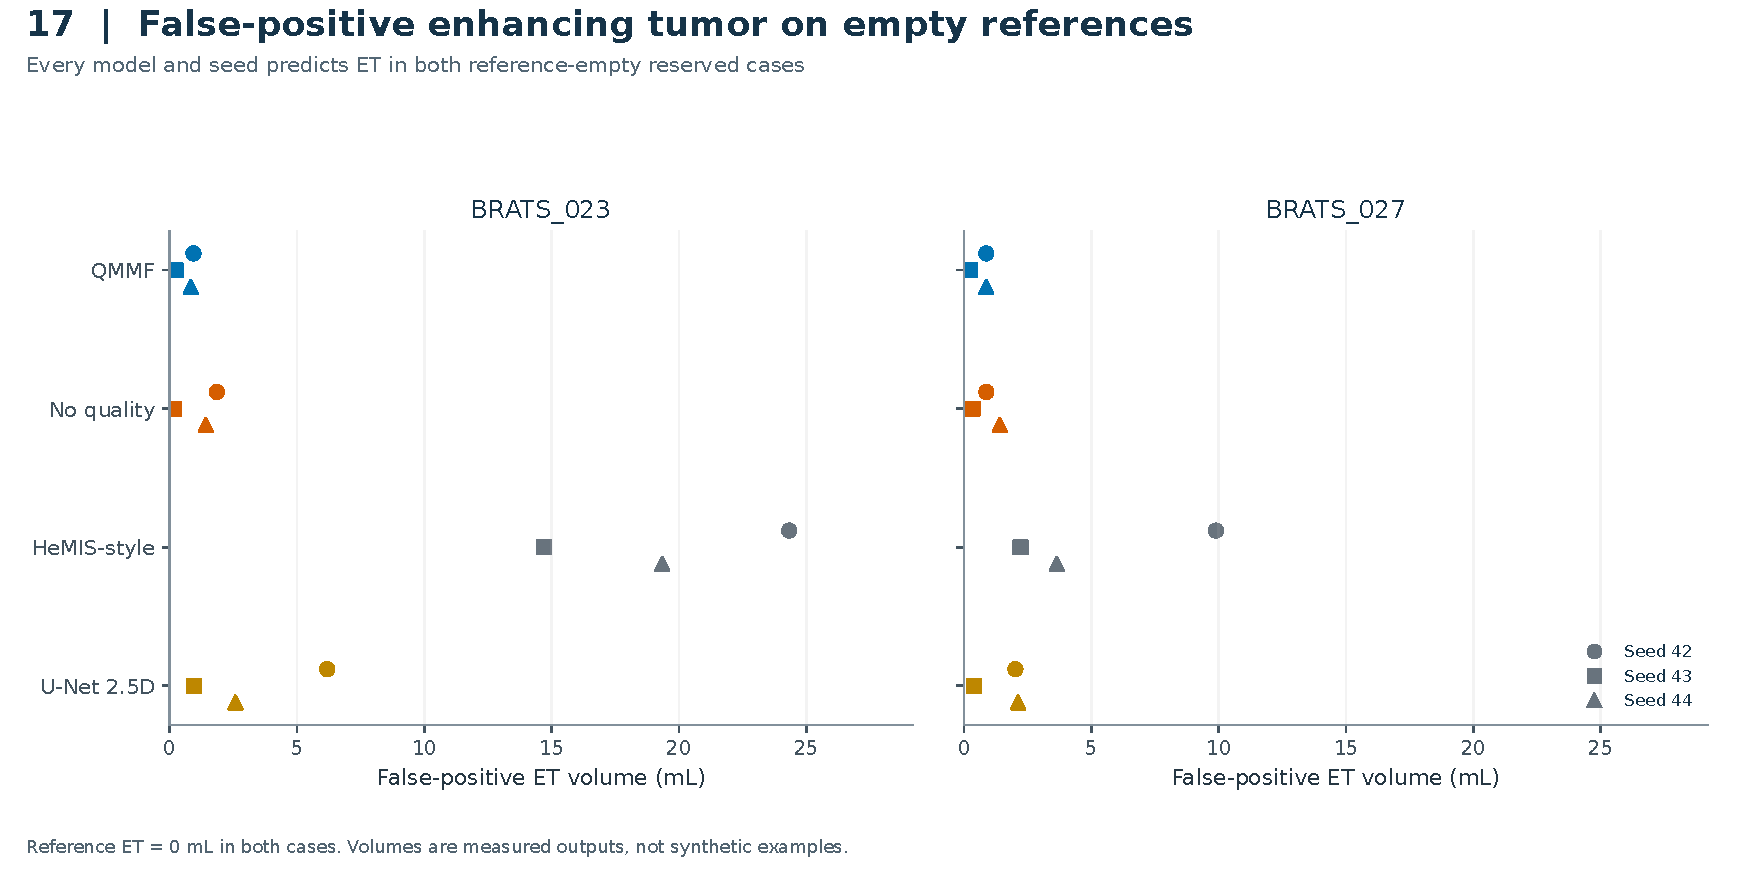
\includegraphics[width=\columnwidth]{figures/fig17_empty_reference_et_failures.pdf}
\caption{Both ET-empty reserved cases (BRATS\_023, BRATS\_027): every model and every seed produced false-positive enhancing-tumour predictions, 24 measured volumes in total.}
\label{fig:etfail}
\end{figure}

The frozen rule excludes empty-reference regions from primary Dice, but both ET-empty reserved cases---BRATS\_023 and BRATS\_027---received false-positive ET predictions from every model and every seed, 24 measured predicted volumes in total (Fig.~\ref{fig:etfail}). Nonempty-reference ET averages must therefore be read together with this failure mode; the observations characterise two cases and do not estimate population specificity. The prespecified qualitative montage retains all four models on BRATS\_143, BRATS\_119 and BRATS\_023 at seed 42, with whole-volume scores displayed; BRATS\_143 carries recorded historical validation exposure, and the montage is illustrative with its original attribution preserved.

\subsection{Historical sensitivity and computation}
\label{sec:sensitivity}

\begin{figure}[htbp]
\centering
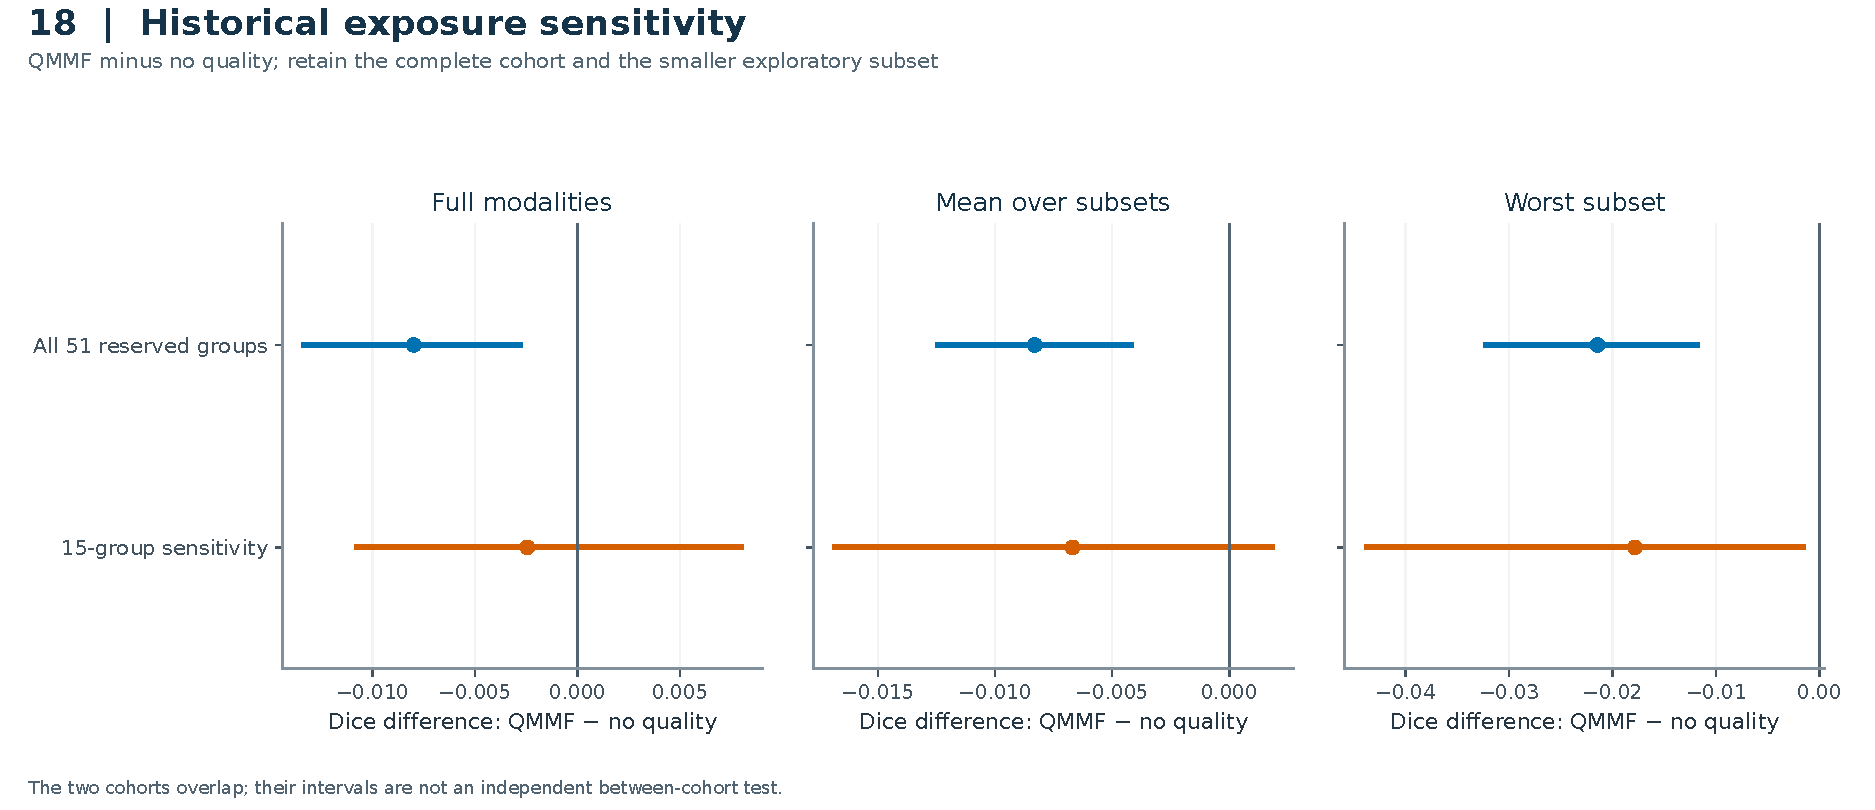
\includegraphics[width=\columnwidth]{figures/fig18_historical_exposure_sensitivity.pdf}
\caption{Complete reserved cohort versus the frozen 15-group historical-exposure sensitivity, all four families and seeds. The sensitivity is a nested subset, not an independent replication.}
\label{fig:sensitivity}
\end{figure}

The exploratory 15-group sensitivity retains all four families and seeds. QMMF-minus-no-quality adjusted intervals cross zero for full-modality and mean-subset Dice; the worst-subset difference remains $-0.0178$ with adjusted interval $[-0.0437,-0.0016]$, still favouring no quality (Fig.~\ref{fig:sensitivity}). Restricting to historically untouched groups therefore weakens but does not reverse the negative finding. On computation, a lossless training-segment cache raised measured throughput by approximately 4.02$\times$ for QMMF and 3.51$\times$ for the HeMIS-style model on Kaggle T4; these bounded measurements use 10 warmup and 100 timed microbatches per model/format and do not estimate end-to-end speedup.

